\documentclass[a4paper,twoside,12pt,DIV=13,BCOR=5mm,numbers=noenddot,cleardoublepage=empty]{scrbook}
\usepackage[utf8]{inputenc}
%======= Einbinden der benötigten Packete (= Zusatzfunktionen)
\usepackage[T1]{fontenc}                % für Fonts in westeuropäischer Codierung
\usepackage{lmodern}										% Latin Modern Paket verändert die verwendete Schriftart. Bessere Darstellung für pdf
\usepackage{textcomp}										% Provides extra symbols, e.g. arrows like \textrightarrow, various currencies (\texteuro,..
\usepackage[latin1]{inputenc}    				% german special characters
\usepackage[english,ngerman]{babel}     % hyphenation   usepackage[english,ngerman]{babel} f. deutsch
\usepackage{pdfpages}										% Einbinden von pdf-Files
\usepackage{pifont,textcomp,mathcomp}   % dingbad psfonts and text-compilant fonts (euro, TM, ...)
\usepackage{amsmath,amsopn,amsthm}      % AMS mathematics
\usepackage{amssymb}                    % zusätzliche Symbole 
\usepackage{xspace}											% avoids eaten spaces

%======= Eine Umgebung für Bilder und Tabellen			  	
%\usepackage[textfont={Small},labelfont={bf},margin=1cm,format=plain,font=singlespacing]{caption}   % hanging caption text [hang]
\usepackage[textfont={small},labelfont={bf},margin=1cm,format=plain,font=singlespacing]{caption}   % hanging caption text [hang]
\captionsetup*[figure]{name=Abb.}			 % Abbildungsunterschrift beginnt mit Abb.
\captionsetup*[table]{name=Tab.}


%======= Farben für Überschriften
\usepackage{color}
\definecolor{TUBlau}{rgb}{0,0.4,0.6}   % TU-blau RGB 0 102 153
\addtokomafont{sectioning}{\sffamily\bfseries\selectfont\color{TUBlau}}
\setkomafont{chapter}{\normalfont\huge\sffamily\bfseries\color{TUBlau}}
\addtokomafont{section}{\Large}
\addtokomafont{subsection}{\normalfont\Large\sffamily\bfseries\color{TUBlau}}
\addtokomafont{subsubsection}{\normalfont\large\sffamily\bfseries\color{TUBlau}}
\addtokomafont{paragraph}{\normalfont\large\sffamily\bfseries\color{TUBlau}}


%======= Kopf-/Fußzeilen
\pagestyle{plain} % nur Fußzeile



%======= Eine kompakte Umgebung für die Bilder
\newcommand{\bild}[4]{{
\begin{figure}[#2]
\begin{center}
\includegraphics[scale=#3]{pictures/#1}
\caption{#4}\label{fig:#1}
\end{center}
\end{figure}
}}


%======= Definitionen eigener Befehle
\newcommand{\degC}{\ensuremath{^{\circ}}C}        % Grad Celsius
\newcommand{\Gu}{\glqq{}}                         % Gänsefüßchen unten
\newcommand{\Go}{\grqq{}\xspace}    												% Gänsefüßchen oben











  			
\usepackage{subscript}
\usepackage{graphicx}
\usepackage{float}
\usepackage{booktabs} % Für schönere Tabellen
\begin{document}
%=============================================================================================
% Titelblatt und Inhaltsverzeichnis
%=============================================================================================
\renewcommand{\baselinestretch}{1.25}
\newcommand{\StudentA}{Marton Harsch}
\newcommand{\MatrNrA}{12123680}
\newcommand{\StudentB}{Michael Malburg}
\newcommand{\MatrNrB}{61806515}
\newcommand{\StudentC}{Jonathan Gamperl}
\newcommand{\MatrNrC}{12302766}

\newcommand{\LUDatum}{22.4.2024}
\newcommand{\LUGruppe}{}
\newcommand{\LUBetreuer}{}

\large
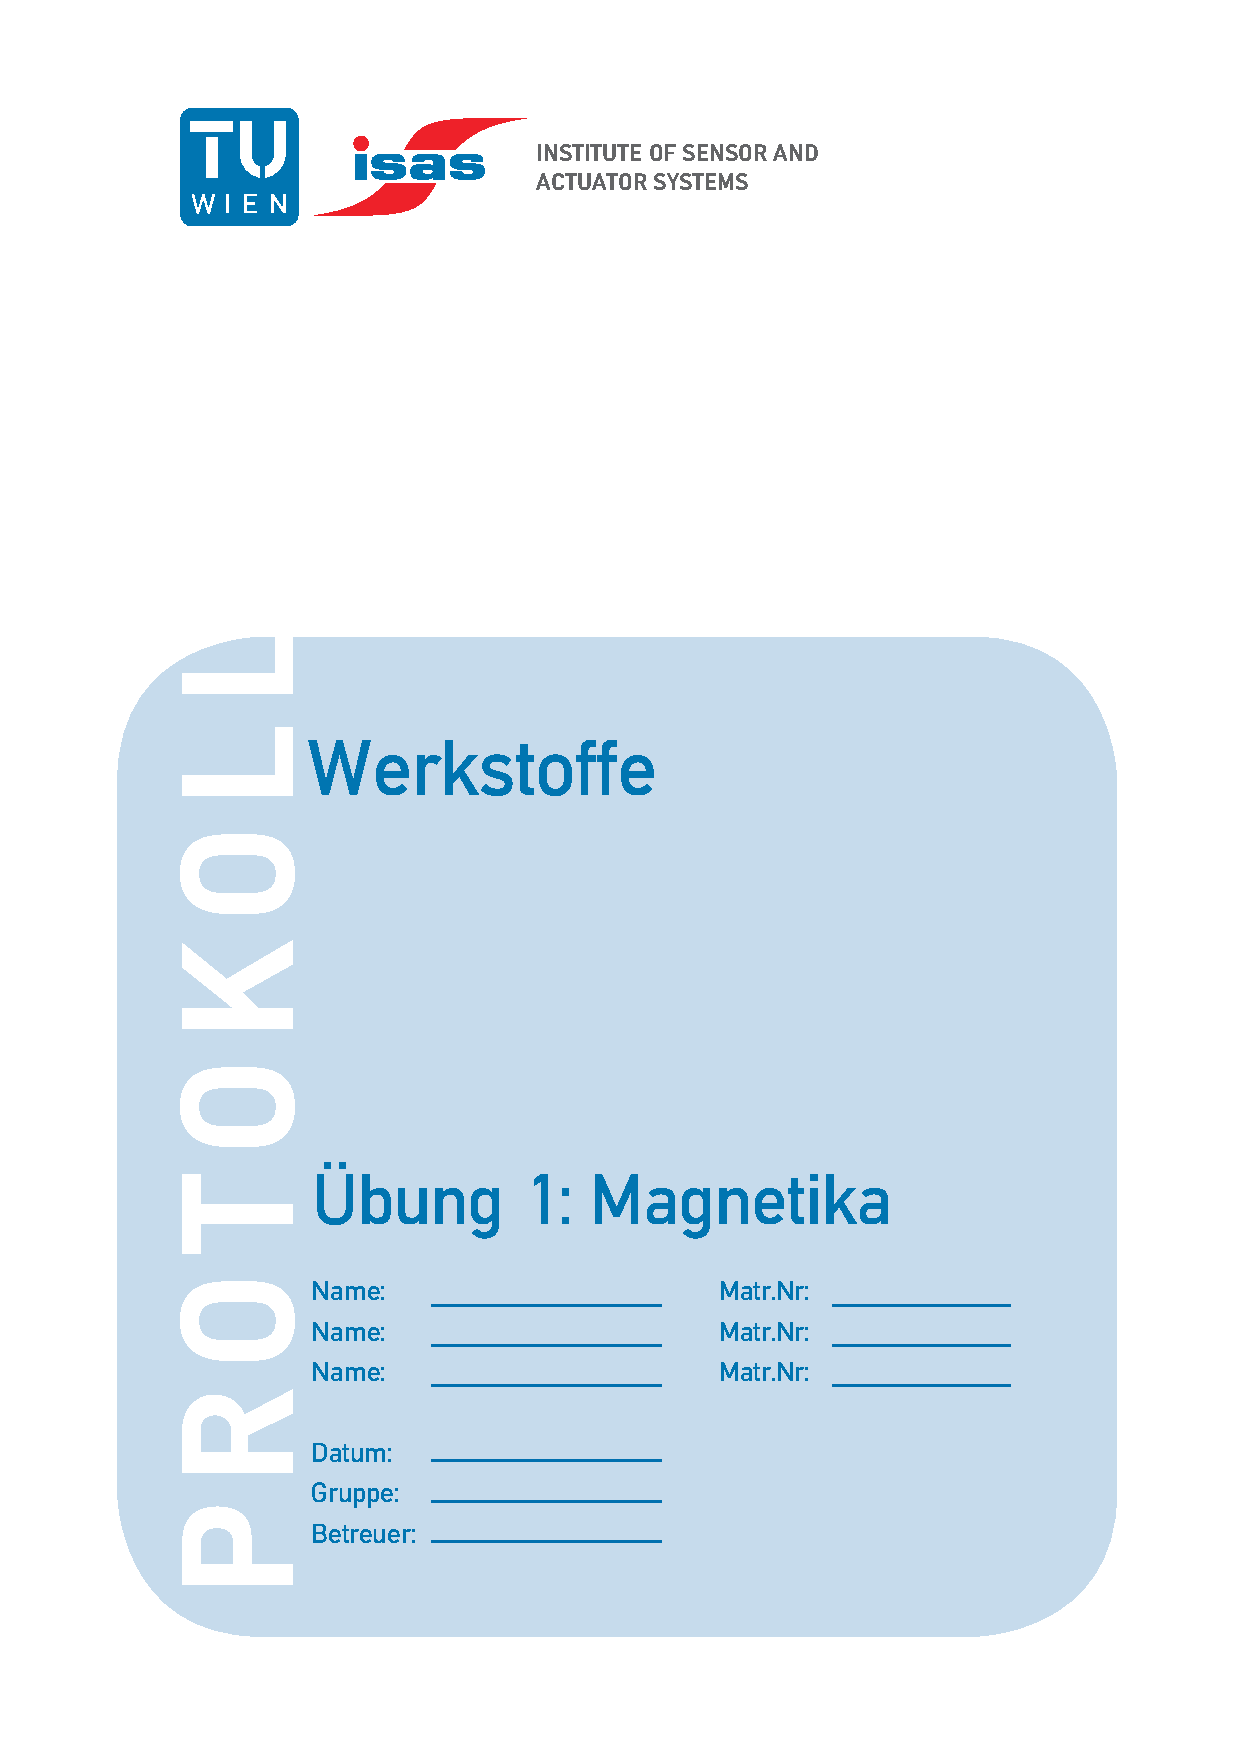
\includepdf[fitpaper=true,
						picturecommand*={\unitlength1cm 
						\put(7.3,7.7){\StudentA} \put(14.1,7.7){\MatrNrA}
            \put(7.3,7.0){\StudentB} \put(14.1,7.0){\MatrNrB}
            \put(7.3,6.3){\StudentC} \put(14.1,6.3){\MatrNrC}
						\put(7.3,5.1){\LUDatum} 
            \put(7.3,4.4){\LUGruppe} 
            \put(7.3,3.7){\LUBetreuer} 
}]
{pictures/DeckblattLUMag}     %file name of title page

\setcounter{chapter}{0}


\chapter{Ringkerntrafo aus unlegiertem Einsatzstahl}
\section{Aufnahme einer Hystereseschleife}

    Die Magnetisierung beschreibt den Zusammenhang zwischen der magnetischen Flussdichte $\Vec{\textbf{B}}$ und der magnetischen Feldstärke $\Vec{\textbf{H}}$
    \begin{equation}
        \Vec{\textbf{B}} = \mu_0 (\Vec{\textbf{H}} + \Vec{\textbf{M}}) = \mu\Vec{\textbf{H}}
    \end{equation} 
    Dabei ist $\mu_0$ die magnetische Feldkonstante und $\mu$ die Permeabilität. \\
    Durch eine Hystereseschleife kann die Beziehung zwischen $\Vec{\textbf{B}}$ und $\Vec{\textbf{H}}$ anschaulich präsentiert werden. Eine typische Hystereseschleife ist eine geschlossene Kurve, die im\textbf{B}-\textbf{H} Koordinatensystem abgebildet wird. \\
    
    \begin{itemize}
        \item  Wenn eine entmagnetisierte Probe bis zur positiven Sättigungsmagnetisierung $+M_S$ aufmagnetisiert wird, wird die \textbf{Neukurve} durchgelaufen. Bei höheren Magnetfeldstärken wird die \textbf{Sättigungspunkt} erreicht, wo die Flussdichte nicht mehr aufsteigen kann.
        \item Wenn das Magnetfeld in die entgegengesetzte Richtung geändert wird, sinkt die magnetische Flussdichte nicht sofort auf Null. Stattdessen bleibt eine Restmagnetisierung im Material zurück. Dieser Punkt wird als \textbf{Remanenzpunkt} bezeichnet mit \textbf{B$_R$}.
        \item Um die Restmagnetisierung zu neutralisieren und das Material vollständig zu entmagnetisieren, muss das entgegengesetzte Magnetfeld eine bestimmte Stärke erreichen. Diese Stärke wird als \textbf{Koerzitivfeldstärke} \textbf{H$_C$} bezeichnet. \\
        
    \end{itemize}
    
    \subsection{Übungsdurchführung}
    
    Im Rahmen der Laborübung war das magnetische Verhalten von unlegierter Einsatzstahl zu bestimmen. Neben der Eisenring wurde noch ein Funktionsgenerator und Integrator mit USB-anschluss zur Verfügung gestellt. Die Hystereseschleifen sind durch dem Integrator erhalten geblieben und könnten durch ein Software am PC zur analyse dargestellt werden.

    \newpage
    
    \subsection{Probe}

    Zur Messung der magnetischen Verhalten von unlegierter Einsatzstahl wurde ein \textbf{Eisen-Ringkern} aus ungeblechter und unlegierter Einsatzstahl bereitgestellt, das mit vier verschiedenen Wicklungen umgewickelt ist.

    \begin{center}
        
    \begin{tabular}{cc}
    Wicklung W1: & 730 Windungen \\
    Wicklung W2: & 749 Windungen \\
    Wicklung W3: & 732 Windungen \\
    Wicklung W4: & 731 Windungen \\
    Kernaußendurchmesser $d_a$ & 183 mm \\
    Kernunnendurchmesser $d_i$ & 153 mm \\
    Breite b & 15 mm \\
    Höhe h & 15 mm \\
    Wirksamer Querschnitt $A_w$ & 225 mm² \\
    Mittlere Eisenlänge $l_m$ & 528 mm \\
    \end{tabular}
    \end{center}
    
    \subsection{Schaltung}

    Es wurden zwei Widerstände und drei Spulen in serie zusammengeschaltet. Beim \textit{$R_2$} wurde die Eingangsspannung \textit{x} gemessen.Auf die vierte Spule wurde die Integrator angeschlossen zur Messung der Ausgangsspannung \textit{y}.
    \begin{figure}[h] 
    \centering
    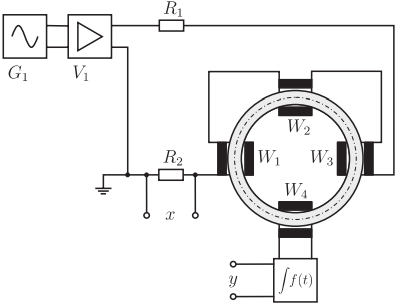
\includegraphics[width=0.5\textwidth]{pictures/HystereseSchaltung.png} % Passe die Breite des Bildes an deine Bedürfnisse an
    \caption{Schaltungsaufbau (Aus Skript)}
    \end{figure}
    \\
    Mit $R_1$ = 4,7$\Omega$, $R_2$ = 1 $\Omega$. \\
    Durch die Funktionsgenerator wurde eine 100 mHz, 20 Vpp Dreiecksignal eingespeist.

    \newpage

    \subsection{Messergebnisse}

        \begin{enumerate}
            \item Die Magnetisierungskurve bei 100 mHz sieht so aus:

            \begin{figure}[h] 
            \centering
            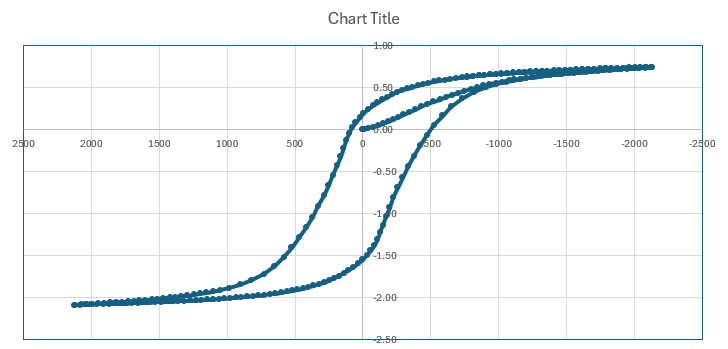
\includegraphics[width=0.5\textwidth]{pictures/50mHz.png} 
            \caption{Hystereseschleife, 50 mHz}
            \label{fig:meinbild}
             \end{figure}

            \\
            
            \item Maßstäbe
                Die Maßstäbe der Achsen müssen aus der Spannungen $U_x$ und $U_y$ bestimmt werden:
                \begin{equation}
                    H = \frac{(N_1 + N_2 + N_3) \cdot I_1}{l_m} \\
                    = \frac{N_1 + N_2 + N_3}{R_2 \cdot l_m} \cdot U_x \\
                    = \frac{A}{V_m} \cdot U_x
                \end{equation}
                \begin{equation}
                    H = 4187.5 \frac{A}{s}
                \end{equation}

                und die magnetische flussdichte B:
                \begin{equation}
                    U_y = -\frac{1}{R \cdot C} \cdot \int U_4 \cdot dt \\
                    = \frac{1}{\tau} \cdot \int N_4 \cdot \frac{d\phi}{dt} \cdot dt \\
                    = \frac{1}{\tau} \cdot N_4 \cdot \phi \\
                    = \frac{1}{\tau} \cdot N_4 \cdot B \cdot A \\
                \end{equation}
                \begin{equation}
                    B = \frac{\tau}{N_4 \cdot A} \cdot U_y \\
                    = 608 \cdot 10^{-3} \frac{T}{V} \cdot U_y \\
                \end{equation}

            \\

            \item Je höher die Frequenz eingestellt ist, desto mehr wird die Hystereseschleife verzerrt. ab einem Punkt werden die Spitzen gar nicht zu beobachten.

            \begin{figure}[h] 
            \centering
            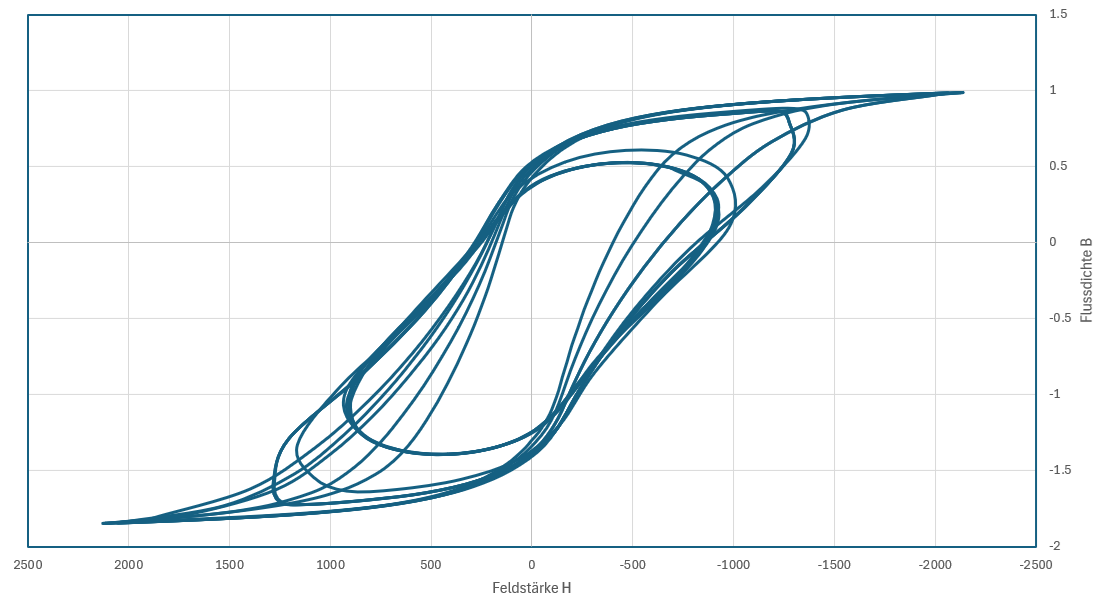
\includegraphics[width=0.5\textwidth]{pictures/freqAnderung.png} 
            \caption{Frequenzänderung mit 100 mHz Schritten}
            \label{fig:meinbild}
            \end{figure}

            Auf dem Abbildung wurde die Frequenz in 100 mHz Schritten erhöht bis zu 1.3 Hz.
            
            \\
            
            \item Bei höheren Frequenzen haben die Magnetfeldänderungen eine größere Wirkung auf das Material. Dies kann zu verstärkten Wirbelstromverlusten führen, insbesondere in leitfähigen Materialien wie Eisenkernen. Diese Verluste beeinflussen die Form der Hystereseschleife und können dazu führen, dass sie breiter wird und die Sättigung des Materials schneller auftritt.

            \\
            
            \item Die frequenz kann als passend betrachtet werden, solange die Spitzen der Magnetisierungsschleife klar erkennbar sind.

            \\
            
            \item eine Rückkopplungsschleife könnte verwendet werden, um den Ausgangsstrom basierend auf einer Referenz zu regeln. Dies kann beispielsweise bei der Regelung von Stromversorgungen oder Verstärkern verwendet werden. Durch eine geeignete Rückkopplung kann der Stromverlauf stabilisiert und linearisiert werden.
            
            \\
            
            \item Anhand der Magnetisierungskurve kann man die Messwerte bestimmen: \\
            \begin{tabular}{cc}
                $B_r$ =& 1.100 T  \\
                $H_c$ =& 256 $\frac{A}{s}$ \\
                $B_{max}$ =& 0.739 T

            \end{tabular}
            
            \\
            
            \item Die magnetische Sättigung in einem Eisenkern  liegt im Bereich von 1,6 bis 2,2 Tesla. Anhand der Hystereseschleife kann man sehen, dass die Flussdichte bei maximaler Feldstärke noch steigen könnte, damit ist Sättigung beim maximalen Strom nicht erreicht

            \\
            
            \item Die maximale Flussdichte ohne der Eisenkern kann durch dividieren mit der spezifischen Permeabilität $\mu_0$ berechnet werden:

                \begin{equation}
                B_{\text{max, ohne Kern}} = \frac{B_{\text{max, mit Kern}}}{\mu_0}
                \end{equation}
    
            \\
            
            \item Die spezifische Verluste sind eng mit der Fläche innerhalb der Magnetisierungskurve verbunden. Die Fläche repräsentiert nähmlich die Energieverluste des Materials pro Volumeneinheit pro Zyklus. Anhand der Plot bsind die spezifischen Verluste ungefähr 1812.5 W/kg.
        
        \end{enumerate}
\section{Aufnahme der Permeabilit\"atskurve}
\subsection{Hintergrund}
Wird aus der Schaltung zur Aufnahme der Hystereseschleife der Integrator entfernt, steht die gemessene Spannung nicht mehr in Proportion 
zum Fluss durch die Spule, sondern zu seiner \"anderungsrate. In diesem Fall kann das Entfernen des Integrators mit dem Ableiten der Funktion
gleichgesetzt werden. Betrachten wir das Verh\"altnis aus der Feldst\"arke und der \"anderungsrate der Flussdichte sprechen wir von 
differenzieller Permeabilit\"at. Wird diese noch durch die Permeabilit\"at des Vakuums geteilterhalten wir die relative differenzielle Permeabilit\"at Ziel ist es diese zu messen 
und mit der Hystereseschleife auf plausibilit\"at zu pr\"ufen, sowie ihren spitzenwert zu finden.
\subsection{Messergebnisse}
\begin{figure}
  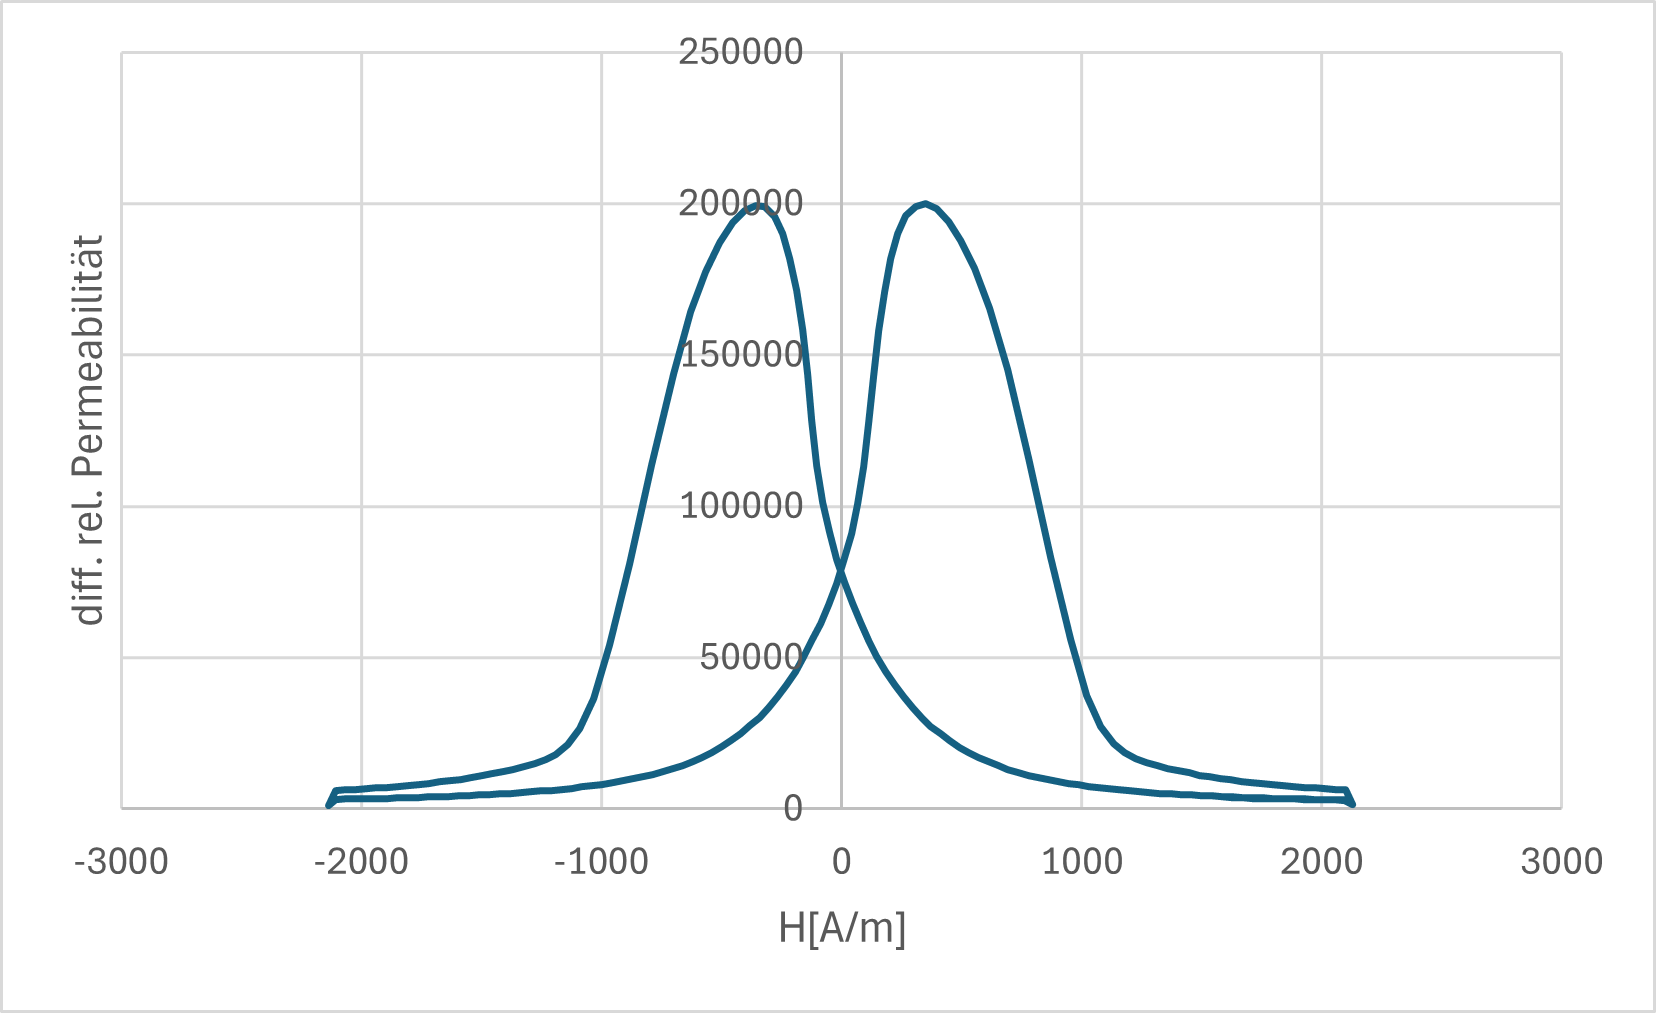
\includegraphics[width=\linewidth]{pictures/Permeabilitaet.png}
  \caption{Differenzielle relative Permeabilit\"at abh\"angig von der Feldst\"arke.}
  \label{fig:perm}
\end{figure}
Das Diagramm \ref{fig:perm} zeigt die gemessene differenzielle relative Permeabilit\"at abh\"angig von der Feldst\"arke. Verglichen mit der Hystereseschleife ist die steigungs\"anderung an sich plausibel, der H\"ochstwert an sich mit fast 200.000 doch etwas fragw\"urdig.

\section{Hysteresefamilie und Entmagnetisierung}
\label{Entmag}
\subsection{Setup}
Um die Neukurve (siehe \ref{Neukurve}) aufnehmen zu k\"ofnnen, braucht es einen unmagnetisierten Werkstoff. 
Der Ringkern wird dazu wiederholt, immer schw\"acher werdend ummagnetisiert wobei die Remanenz jedes mal kleiner wird.
Die dabei entstehende zusammensetzung aus schw\"acher werdenden Hystereseschleifen wird als Hystesresefamilie bezeichnet. 
Um einen kontinuierlich schw\"acher werdenden Sinusstrom durch die Elektromagneten zu schicken wird das Signal des Funktionsgenerators 
mit der Spannung eines sich entladenden Kondendsators moduliert. Der Funktionsgenerator liefert unmoduliert eine Sinusspannung von 6Vpp mit einer Periodendauer von 10s.
Die RC Schaltung mit deren Spannung die des Funktionsgenerators moduliert wird besitzt eine Zeitkonstante von 60s. Die  induzierte Spannung an der Messpule wird f\"ur diese Messung integriert. 
Die Widerstandswerte bleiben gleich.
\subsection{Messergebnisse}
\begin{figure}
  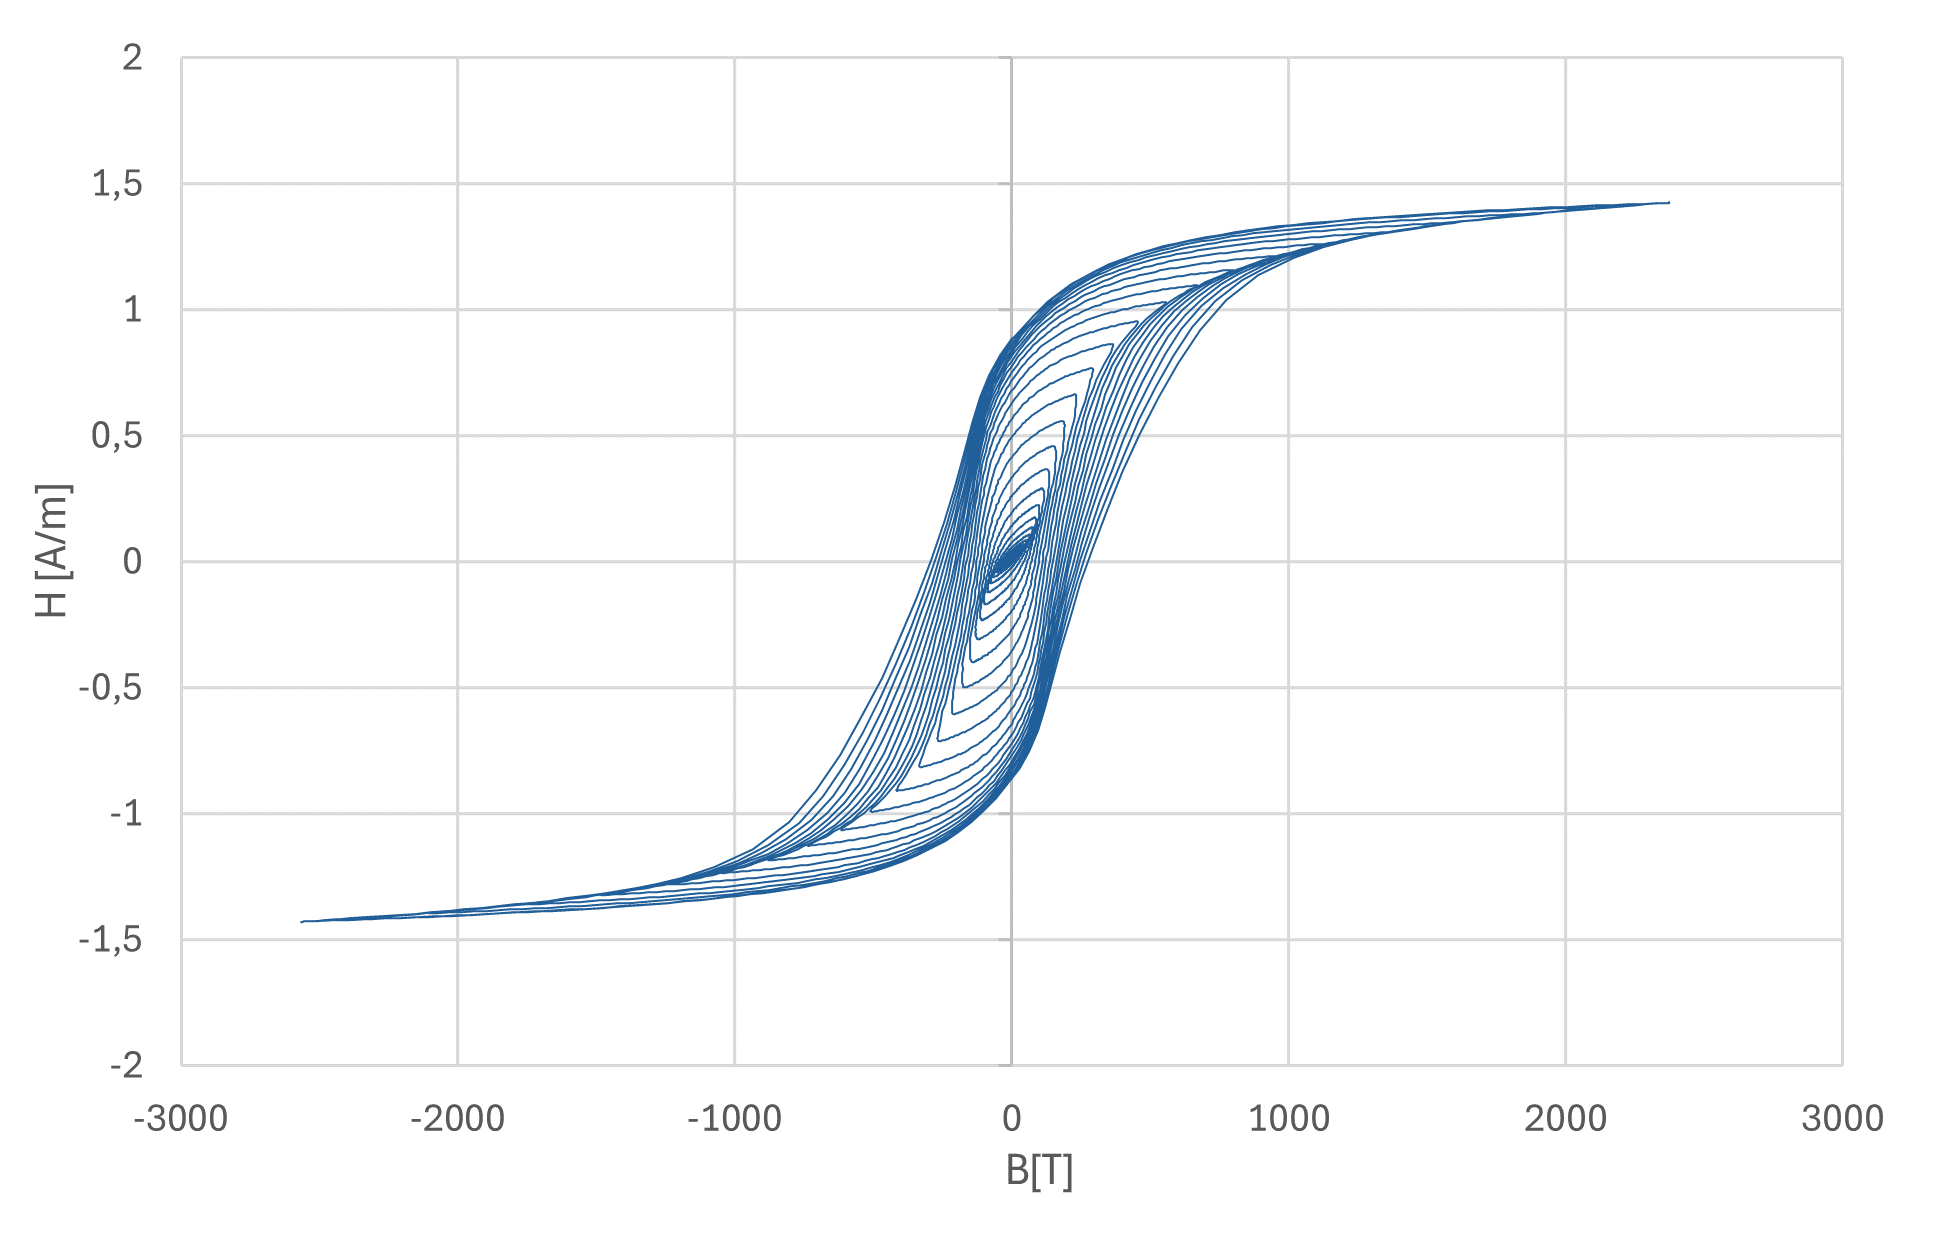
\includegraphics[width=\linewidth]{pictures/Hysteresefamilie.png}
  \caption{Hysteresefamilie die die Entmagnetisierung des Ringkerns zeigt.}
  \label{fig:entmag}
\end{figure}
In dem Diagramm \ref{fig:entmag} kann sch\"ofn die Entmagnetisierung des Materials durch die immer kleiner werdenden Hystereseschleifen betrachtet werden.

\section{Die Neukurve}\label{Neukurve}
\subsection{Setup}
Ziel dieser Messung ist es eine Hystereseschleife inklusive einer Neukurve aufzunehmen. 
Dazu wird der gleiche Messaufbau wie beim einfachen Messen der Hystereseschleife verwendet. Anders ist in diesem Fall aber, dass der Kern des Trafos entmagnetisiert wurde (siehe \ref{Entmag}) und 
die Dreiecksspannung nur als zwei Zyklen Burst angelegt wird.
\subsection{Messergebnisse}
\begin{figure}[H]
\centering
  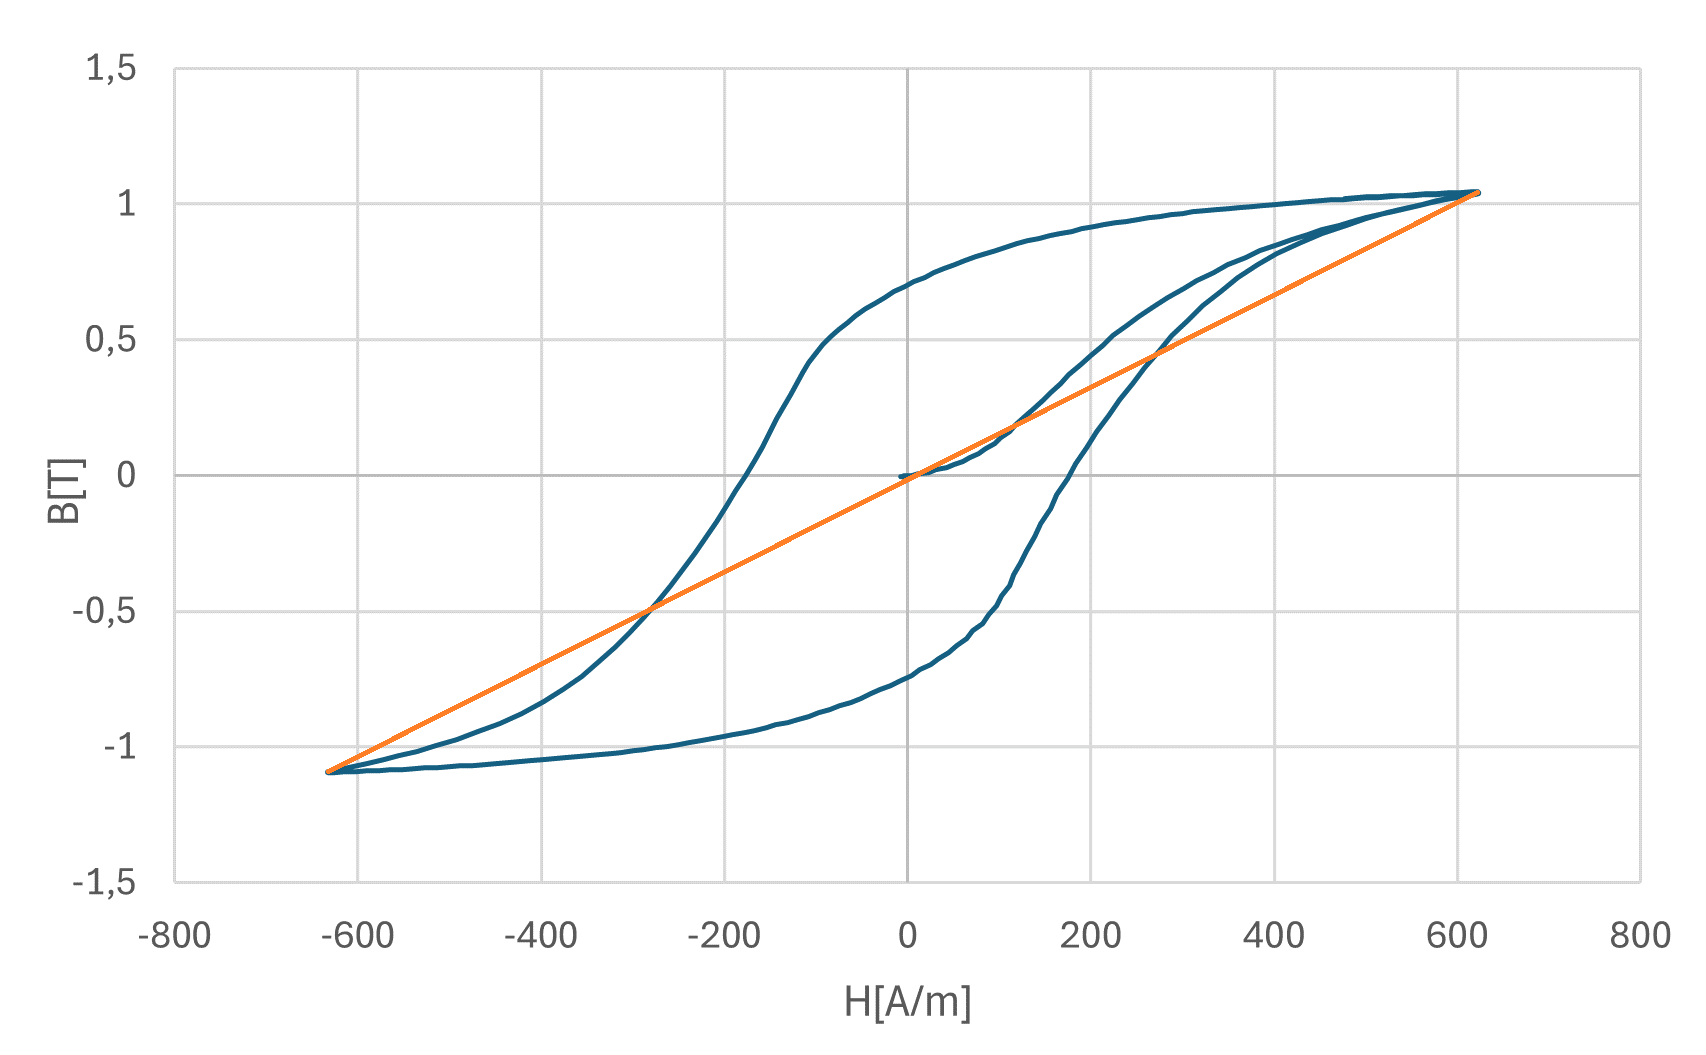
\includegraphics{pictures/Neukurve.png}
  \caption{Hystereseschleife mit Neukurve.}
  \label{fig:neukurve}
\end{figure}
Im Diagramm \ref{fig:neukurve} sehen wir die bereits bekannte Hystereseschleife mit einer zus\"atzlichen Neukurve die das initale Magnetisieren des unmagnetisierten Stoffes darstellt.
\chapter{Übungen am Elektromagneten}
\section{Metallscheiben im Magnetfeld}
\label{Metallscheiben im Magnetfeld}
\subsection{Aufgabenstellung}
\noindent\\
Der Abstand der Polschuhe wurde auf 6\,mm, der Strom auf 30\,A eingestellt.
Es wurden dann verschiedene Metallscheiben aus Al, Cu und Messing (jeweils 20 bzw. 30 mm Durchmesser und eine Dicke von 2 mm) durch den Luftspalt fallengelassen, wie in Abb. \ref{fig: Metallscheiben} zu sehen ist.

\begin{figure}
    \centering
    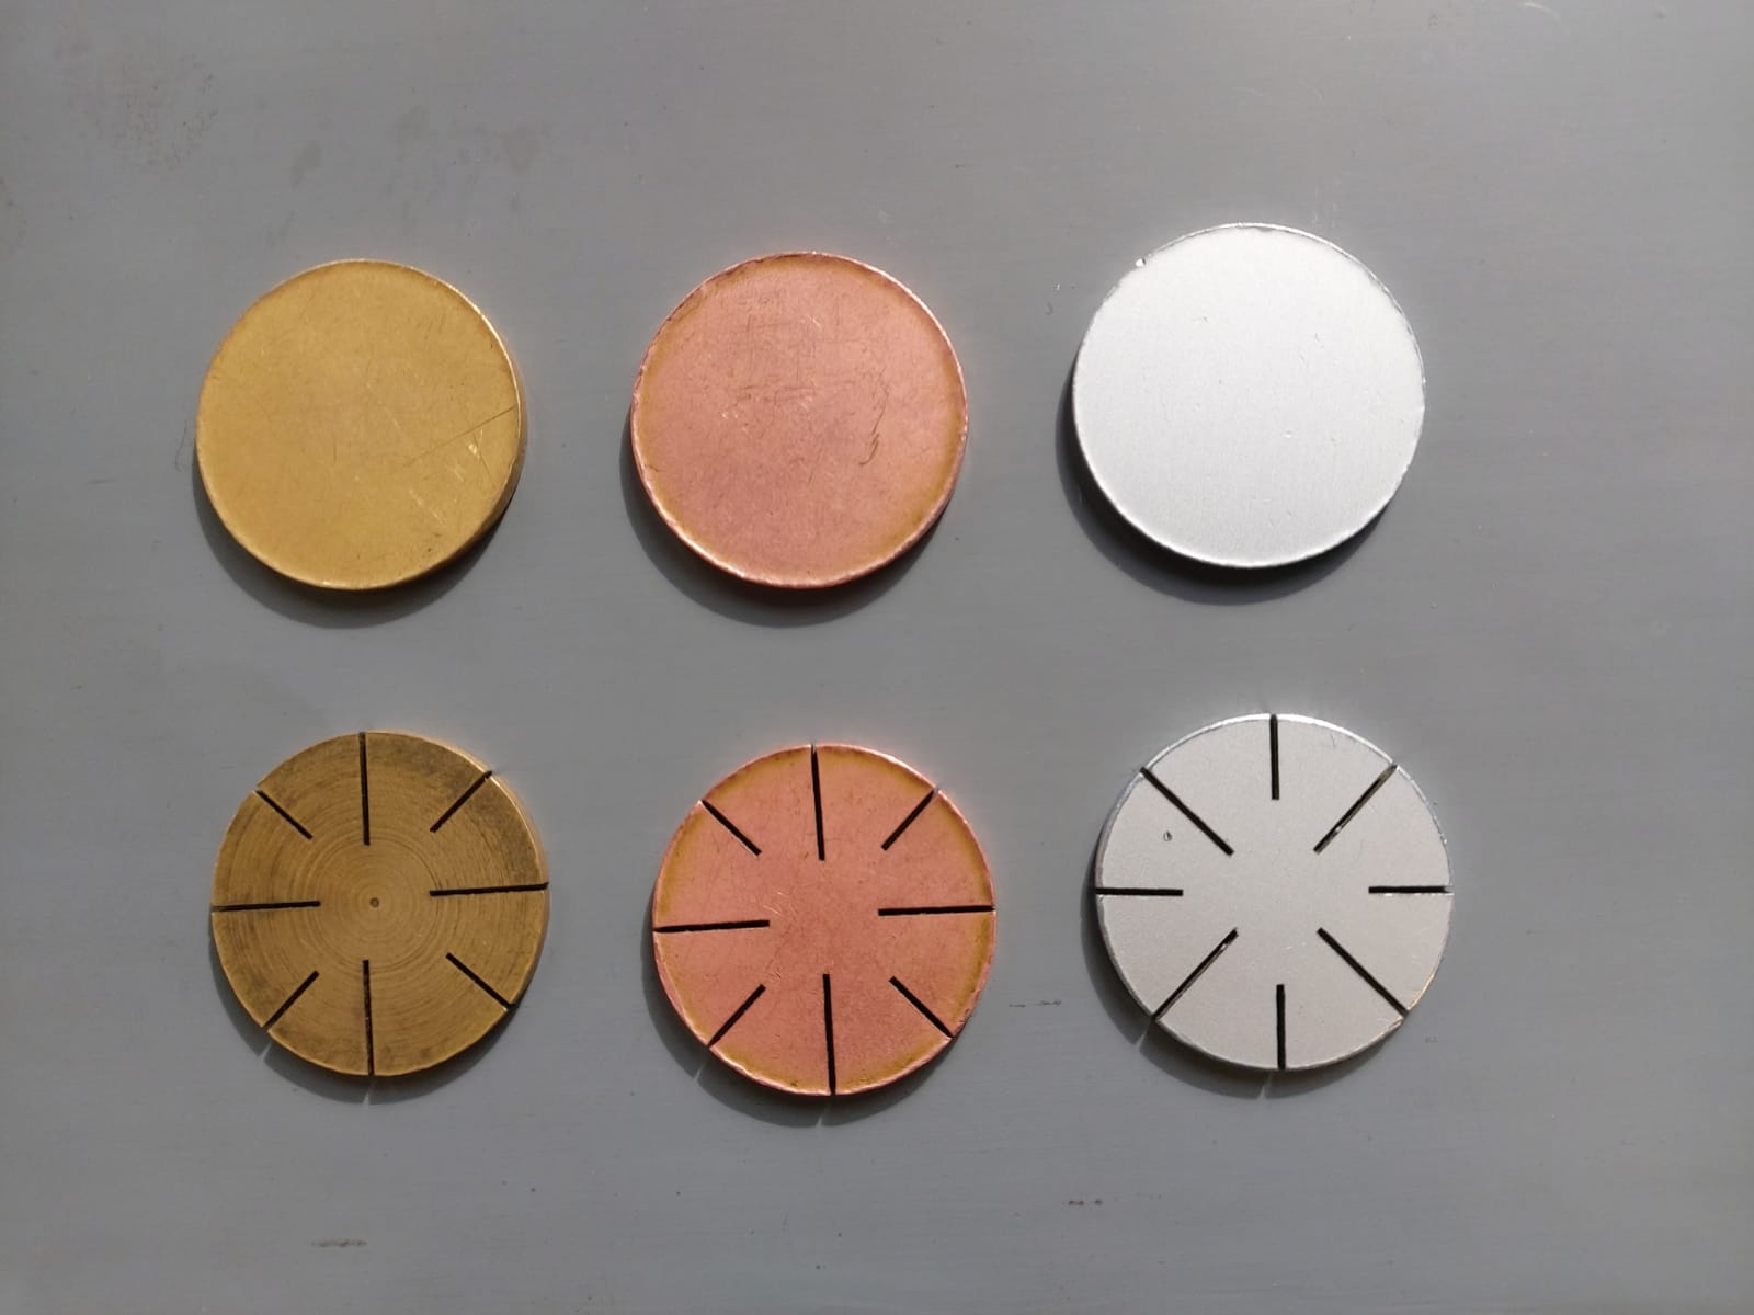
\includegraphics[scale=0.4]{pictures/Metallscheiben.pdf}
    \caption{Die für den Versuch \ref{Metallscheiben im Magnetfeld} verwendeten Metallscheiben.}
    \label{fig: Metallscheiben}
\end{figure}
\subsection{Aufgabenstellung und Ergebnisse}
Die Münzen wurden durch den Luftspalt der Magnete fallen gelassen. Dabei wurde beobachtet, dass der Fall der Münzen stark abgebremst wird, nachdem diese das Magnetfeld durchquert haben und sich die vom homogenen Feld durchsetzte Fläche wieder ändert. Es wirkt also eine bremsende Kraft auf die Münze, die von den induzierten Spannungen und den daraus resultierenden Wirbelströmen herrührt. Die Wirbelströme erzeugen für sich ein Magnetfeld, welches dem äußeren entgegenwirkt. Das das Magnetfeld homogen und konstant ist, tritt der Effekt nur bei (Ein- und) Austritt aus dem Feld auf. 

\noindent Die Stärke der Wirbelströme ist vom Ohmschen Gesetz (\ref{OhmschesGesetz}) bestimmt und hängt von den Leitfähigkeiten $\sigma_i$ der Materialien ab.

\begin{equation}
	I = \frac{U}{R}
	\label{OhmschesGesetz}
\end{equation}
mit 
\begin{equation}
    R = \frac{l}{\sigma_i*A}.
    \label{SpezifischerWiderstand}
\end{equation}

\noindent A stärksten wurde die Aluminium-Münze gebremst, dann kam die Kupfer-Münze, am wenigsten war der Effekt bei Messing zu beobachten. Die Münzen mit den radialen Einkerbungen wurden deutlich schwächer gebremst. Grund dafür ist, dass die Flächen, die vom Magnetfeld durchsetzt werden, voneinander getrennt sind, sodass so jeweils betragsmäßig kleinere Spannungen im Metall induziert werden. 

\noindent Der Versuch sollte mit einer 5-Cent-Münze wiederholt werden. Da diese nur mit einer dünnen Schicht Kupfer überzogen ist, unter welcher sich ein Eisenkern verbirgt, war ein anderer Verlauf des Experiments zu erwarten. Tatsächlich ließ die ferromagnetische Eigenschaft von Eisen die Münze sofort an der Magneten haften, und gar nicht erst durch den Luftspalt fallen.

\noindent Im letzten Teil des Abschnitts wurde eine 1cm dicke, großflächige Alluminiumplatte zwischen die Magneten geschoben. Diese überragte dabei den gesamten Rand des Luftspaltes, an welchem ein inhomogenes Magnetfeld vorliegt. Bei ruckartigen Bewegungen der Platte war die von den Wirbelströmen ausgehende Kraft am größten, und die Platte konnte am einfachsten wieder mit langsamer Bewegung entfernt werden.

\section{Eisenblech im Magnetfeld}
\subsection{Aufgabenstellung}
Es sollten rotierbare Plättchen aus Weißblech bzw. Trafobleche in das Magnetfeld eingebracht werden, sodass die Drehachse normal auf das Feld steht (Abb. \ref{fig: RottierbarePlaettchen}). Der Einfluss der Walzart der Bleche sowie ihrer Form auf ihre Ausrichtung im Magnetfeld wurde untersucht. 
\begin{figure}
    \centering
    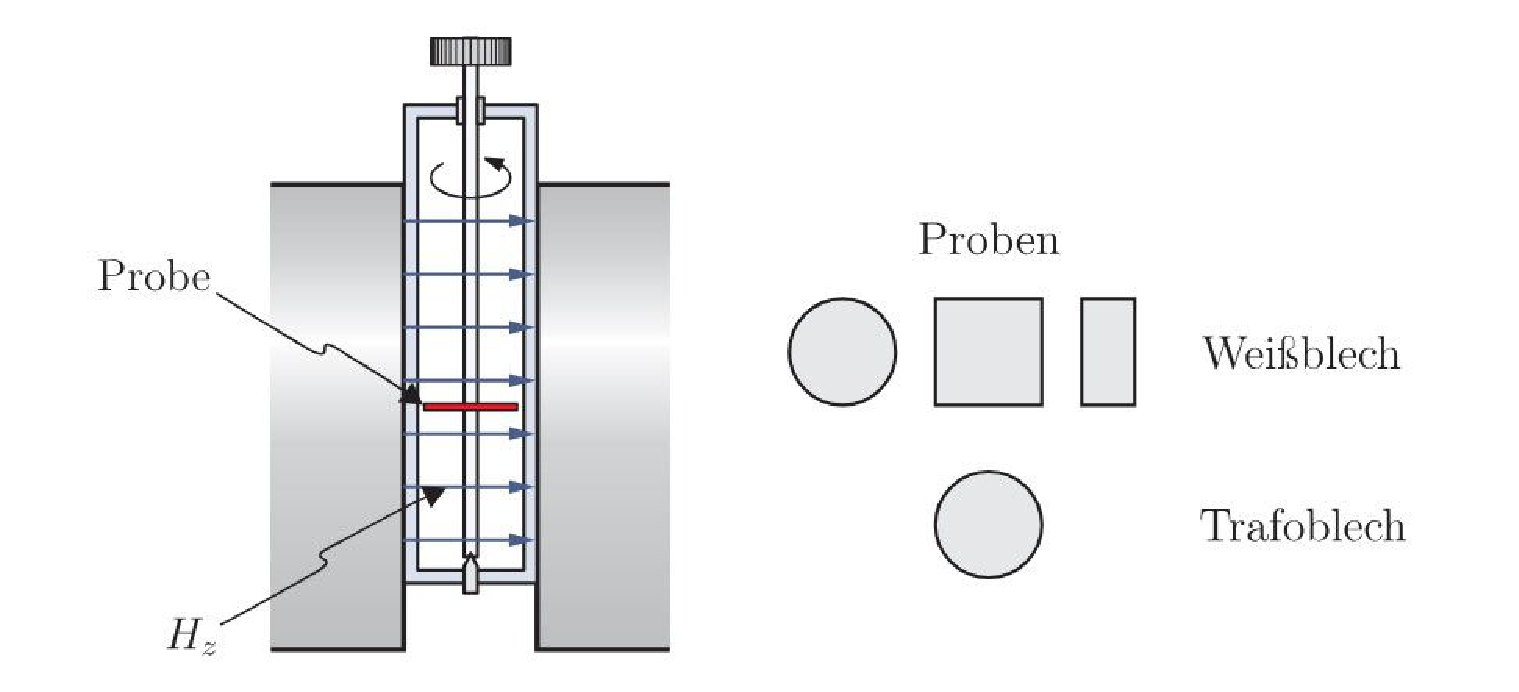
\includegraphics[scale=0.5]{pictures/Anordnung Blechproben.pdf}
    \caption{Anordnung zum Versuch an den Blechplättchen und die vier Versuchsplättchen.}
    \label{fig: RottierbarePlaettchen}
\end{figure}

\subsection{Versuchsdurchführung und Ergenisse}
\noindent Auf der Achse waren die 4 Plättchen drehbar befestigt. Grundsätzlich gilt, dass der magnetische Fluss den Weg des geringsgten magnetischen Widerstandes einschlägt. Das quadratische Plättchen aus Weißblech wies daher vier stabile Ruhelagen auf, bei denen die Querdiagonalen von einem Polschuh zum anderen zeigten. Wurde das Plättchen aus einer dieser Ruhelagen gedreht, versuchte es sich in jene Ruhelage zurückzurichten, welche die geringste Rotation erforderte. Das rechteckige Weißblechplättchen richtete sich ebenso so aus, dass der Abstand Blech zu Magnet minimiert wurde unter Einbehaltung der Symmetrie: daher drehten sich die kürzeren Seiten in Richtung der Polschuhe. Das runde Weißblechplättchen wies keine besondere Vorzugsrichtung im Feld auf, was an seiner Rotationssymmetrie liegt. Im Gegensatz dazu besaß das runde Trafoblech 2 um 180° verdrehte Ruhelagen. Das liegt daran, dass das sogenannte "kornorientierte Elektroblech" in eine bestimmte Richtung gewalzt wird, sodass die Kristallkörner des Legirungsmaterials eine Vorzugsrichtung einnehmen. Das führt zu einem geringeren magnetischen Widerstand für ein Feld in dieser Richtung.
\section{Diamagnetische Stoffe}
Bei diesem Versuch wurden vier Proben jeweils an einem Faden befestigt. Dabei handelte es sich um Platin und Titan, zwei paramagnetische Stoffe, sowie die diamagnetischen Stoffe Wismut und pyrolathischen Graphit. Am Faden hängend wurden die Proben in das Magnetfeld geführt. Der pyrolathische Graphit wies die größte Richtungsabhängigkeit aus, und zwar stellte sich das Plättchen stets parallel zu der Fläche der Polschuhe. Ein ähnliches Verhalten war bei Platin zu beobachten. Hingegen reagierten Titan und Wismut nicht merklich auf das magnetische Feld, was wegen der betragsmäßig deutlich kleineren Suzeptilitäten der Materialen nicht sonderlich überrascht. (siehe Tabelle \ref{tab: sus} für typsiche Werte der Suszeptilitäten).

\begin{table}[h]
    \centering
    \begin{tabular}{@{}lcc@{}}
    \toprule
    Material & Magnetische Suszeptibilität (\(\chi_m\)) & Typ \\
    \midrule
    Platin & \(2.63 \times 10^{-4}\) & Paramagnetisch \\
    Titan  & \(1.80 \times 10^{-4}\) & Paramagnetisch \\
    Wismut & \(-1.66 \times 10^{-4}\) & Diamagnetisch \\
    Pyrolytischer Graphit & \(-4.00 \times 10^{-4}\) & Diamagnetisch \\
    \bottomrule
    \end{tabular}
    \caption{Magnetische Suszeptibilitäten verschiedener Materialien}
    \label{tab: sus}
\end{table}

\section{Messung des Magnetfeldes}
Zur Messung des magntischen Feldes wurde ein Gauss/Teslameter, Model 5080 der Firma F.W. BELL, verwendet, welches direkt in der Lage ist, die magnetische Flussdochte zu messen. Einzig war darauf zu achten, das Messgerät richtig zu kalibrieren. Bei dem Kalibrierungsmagneten ergab die Messung $-4.47 mT$, was den Messfehler darstellte.

\begin{figure}[H]
    \centering
    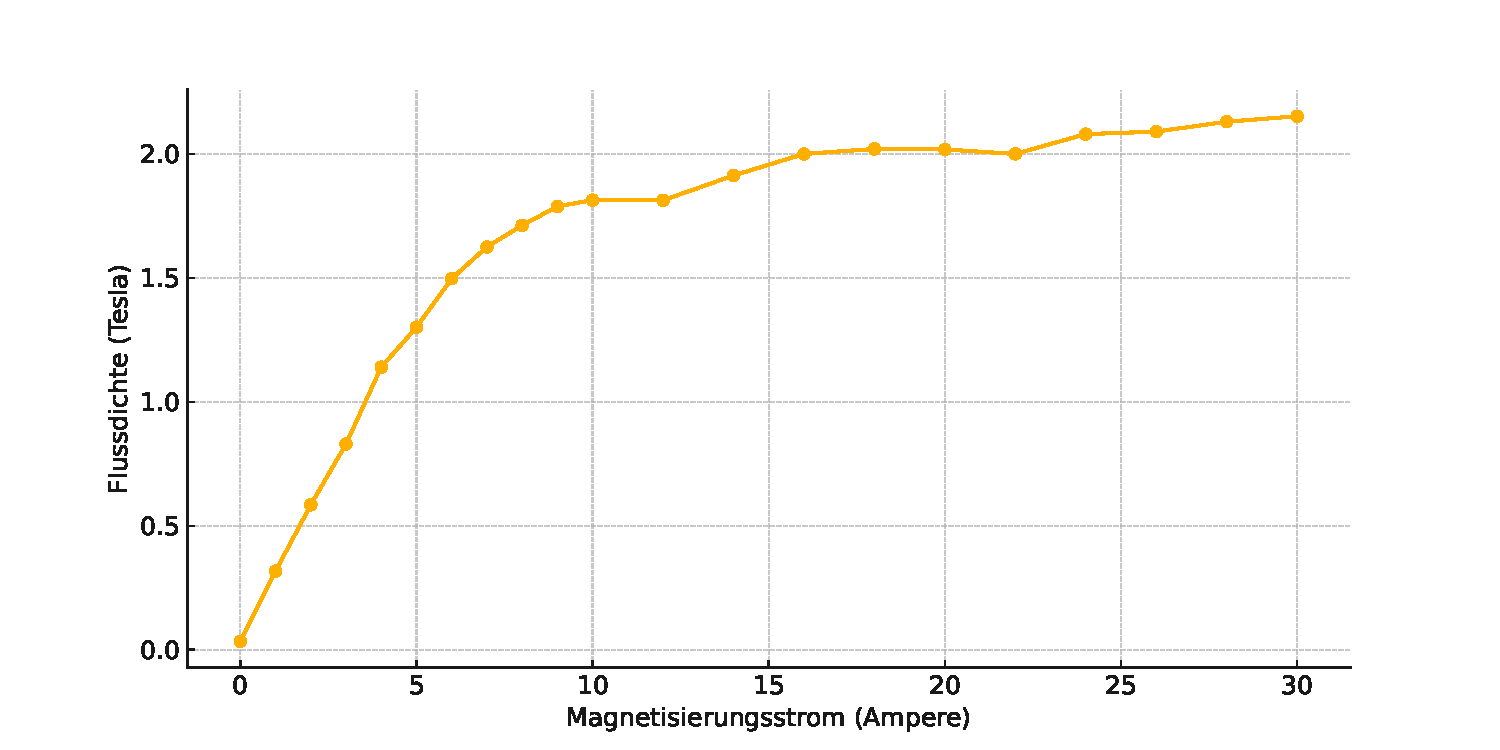
\includegraphics[width=0.8\textwidth]{pictures/Flussdichte_Strom_Plot_Updated.pdf}
    \caption{Flussdichte in Abhängigkeit des Magnetisierungsstroms.}
    \label{fig:flussdichtestrom}
\end{figure}

\noindent Abbildung \ref{fig:flussdichtestrom} zeigt die Messergebnisse. Es ist eine Remanenzflussdichte von $34.5 mT$ bei einem Magnetisierungsstrom von $0 A$ gemessen worden. Weiters ist zu erkennen, dass das Material bei etwa $15-20 A$ gesättigt ist, ab da steigt die Flussdichte nur noch leicht über 2 Tesla an.

\section{Lorentzkraft}
Es wurde ein mit $20 A$ druchflossener Leiter in das Magnetfeld gelegt. Auf den Leiter wirkte die Lorentzkraft entsprechend \autoref{Lorentzkraft}, die ihn nach oben oder unten (je nach Positionierung des Drahtes) zog. Bei einem Magnetisierungsstrom von $20 A$ beträgt die Flussdichte zwischen den Polschuhen 2 Tesla, das entspricht einer Kraft von 4\,N auf den Leiter.
\begin{equation}
	\mathbf{F} = \mathbf{B} \times I \mathbf{e_i} \cdot l
	\label{Lorentzkraft}
\end{equation}
\end{document}